\RequirePackage{plautopatch}
\documentclass[luatexja,fontsize=12pt]{jlreq}\usepackage{ifthen}\newcounter{enlarge}\setcounter{enlarge}{1}
%\documentclass[luatexja,fontsize=18pt]{jlreq}\usepackage{ifthen}\newcounter{enlarge}\setcounter{enlarge}{2}
%\documentclass[luatexja,fontsize=22pt]{jlreq}\usepackage{ifthen}\newcounter{enlarge}\setcounter{enlarge}{3}
%%%%%%
\usepackage{xcolor}
\usepackage{hyperref}
\hypersetup{colorlinks=false,citebordercolor=green,linkbordercolor=red,urlbordercolor=cyan,}
\usepackage{amsmath}
\usepackage{amssymb}
\usepackage{framed}
\usepackage{ulem}
\usepackage{wrapfig}
\usepackage{graphicx}
\usepackage[font=small]{caption}
\usepackage{enumerate}
%%%%%%
\newcommand{\LS}[2]{\ifthenelse{\value{enlarge}=2 \OR \value{enlarge}=3}{#1}{#2}}
\newcommand{\LO}[1]{\LS{#1}{\relax}}
\newcommand{\SO}[1]{\LS{\relax}{#1}}
\newcommand{\LNL}{\LO{\notag\\&}}
%%%%%%
\newtheorem{eg}{例}
%%%%%%
\begin{document}
\begin{flushright}
\today \\
TAIYO
\end{flushright}

{\Large%
\noindent
\textbf{%
数学A 1章「場合の数と確率」 2節「確率」 レジュメ
\LO{\\ \color{teal} 〈拡大版〉}}
}

{\footnotesize%
\mbox{}\\

}
\begin{quotation}
授業スライドはつくったが\footnote{%
スライドは\url{https://github.com/sodesudesu/HS-Math}
で公開している。
また、本資料の拡大版(22pt)もダウンロードできる。
高校生が電車やバスでの通学中にスマートフォンなどの小さな画面で予習をするのに役に立つと思う。}、それだけだと何をしゃべる必要があるか分からないので、カンペとしてここに記録しておく。
だから、これは誰かに読んでもらうために書いた訳ではない(←こう言っとけば何でも許されると思っているのだろうか)。

脚注に書いたことは、特に質問がなければ説明しない。
\end{quotation}

\section*{(準備)集合}

確率では事象を集合で表すので、必要な集合の知識(だけ)を整理しておく。
\mbox{}\\

\paragraph{基本的な記号の整理}\mbox{}\\
\indent
ここでは、集合をアルファベット大文字で、要素をアルファベットの小文字で表す。

$a$が集合$A$の要素であれば、
\begin{align} \label{eq:0_1}
a \in A (A \ni a~も同じ)
\end{align}
と表す。

集合$A$が集合$B$の部分集合であれば、
\begin{align} \label{eq:0_2}
A \subset B (B \supset A~も同じ)
\end{align}
と表す。

集合$A$と集合$B$のどちらにも属する要素全体の集合を共通部分といい、
\begin{align} \label{eq:0_3}
A \cap B
\end{align}
と表す。
また、$A$と$B$の少なくとも一方に属する要素全体の集合を和集合といい、
\begin{align} \label{eq:0_4}
A \cup B
\end{align}
と表す。

全体集合は$U$で表す(確率では全事象をこれで表す)。

空集合は$\varnothing$で表す(確率ではこれで空事象を表す)。
\mbox{}\\

\paragraph{要素の個数}\mbox{}\\
\indent
有限個の要素からなる集合$A$について、その要素の個数を$n(A)$で表す。

有限集合$A$と$B$に対して、
\begin{align} \label{eq:0_5}
n(A \cup B)=n(A)+n(B)-n(A \cap B)
\end{align}
が成り立つ。
$A \cap B=\varnothing $であれば(確率では排反事象にあたる)、(\ref{eq:0_5})の右辺第3項が0なので、
\begin{align} \label{eq:0_6}
n(A \cup B)=n(A)+n(B)
\end{align}
と、よりシンプルな表式が得られる。
\mbox{}\\

\paragraph{補集合}\mbox{}\\
\indent
全体集合$U$の部分集合$A$について、補集合は$\overline{A}$で表す。
ここで、
\begin{align} \label{eq:0_7}
\overline{\overline{A}}=A
\end{align}
が成り立つ。
$A$の補集合の補集合は$A$にもどる、という意味である。

ここまでに紹介した集合をベン図で表したものを図\ref{f:0.1}に示した。
\begin{figure}[] 
\centering 
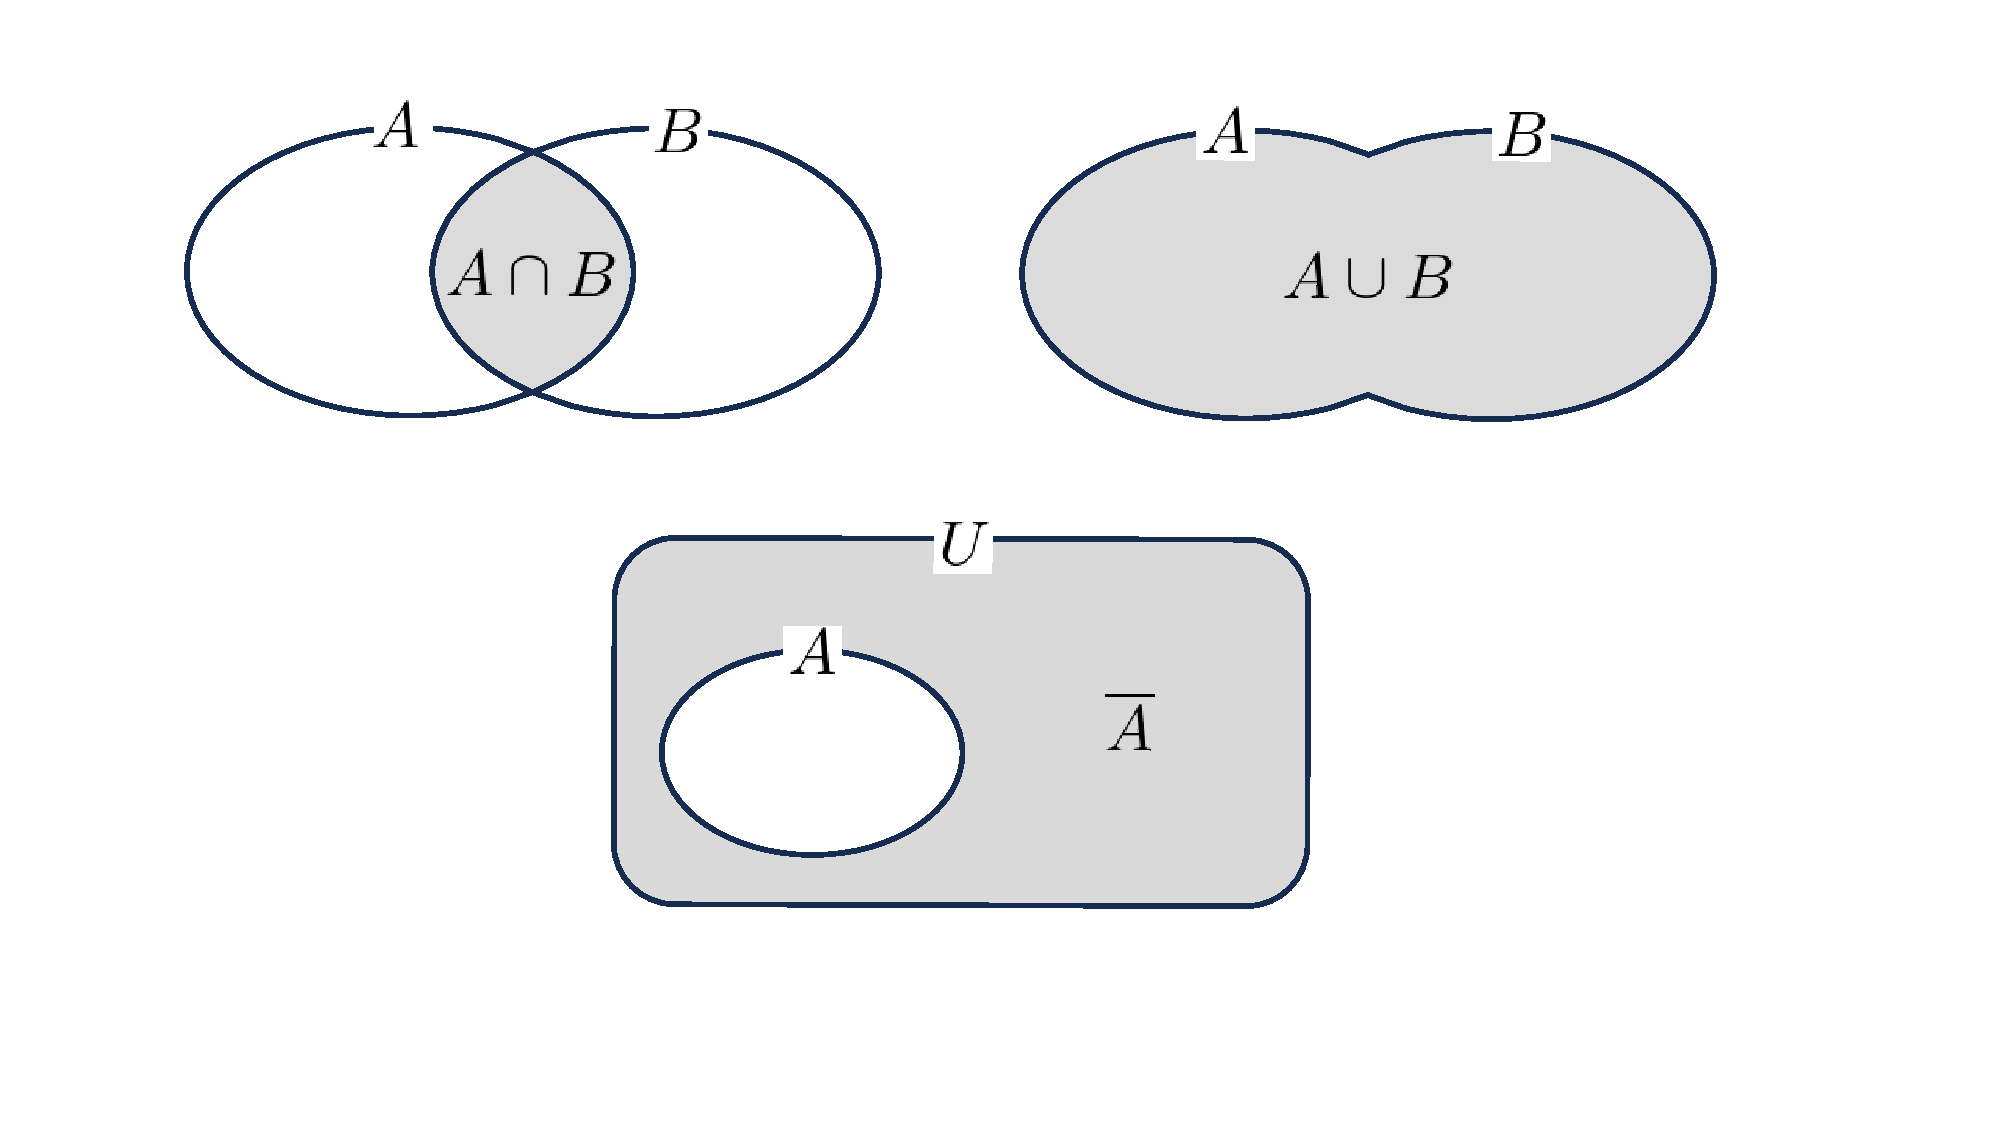
\includegraphics[width=10truecm]{f0_1.pdf}
\captionsetup{width=.9\linewidth}
\caption{%
説明した集合のベン図。
}
\label{f:0.1}
\end{figure}%

\section*{6 事象と確率}

\subsection*{A 確率の意味}

ある事柄が起こることが期待される程度を数値で表したものを\textbf{確率}という。
%例えば「コインを投げて表が出る確率は1/2」と言ったら、何度も何度も繰り返しコインを投げたとき、表が出る回数がその半分になることを意味している。
当然のことだが、「コインを投げて表が出る確率は1/2」と言ったら、2回投げれば必ず1回は表、1回は裏がでるという意味ではない(確率の意味については\pageref{fn:1}ページの脚注\ref{fn:1}も見よ)。
%ココらへんで10人に9人が死ぬ病気の話をしたい。

\subsection*{B 試行と事象}

同じ状況のもとで繰り返すことができ、結果が偶然によって決まる実験や観測などを\textbf{試行}といい、その結果起こる事柄を\textbf{事象}という。

ある試行を考えるとき、はじめに、起こりうる結果全体の集合$U$を指定し、この試行により起こりうる事象を$U$の部分集合で表す。

このように、確率では事象を集合を用いて表す。
ところで、$U$で表される事象を\textbf{全事象}と呼ぶ。
また、$\varnothing$で表される事象を\textbf{空事象}という。

$U$の1つの要素からなる集合で表される事象を\textbf{根元事象}という。

\begin{eg}[1つのサイコロを投げる試行における事象]
1つのサイコロを投げる試行を考える。
サイコロの1の目が出たことを数字の1で表すことにすれば、全事象は
\begin{align} \label{eq:6.1}
U= \{ 1, 2, 3, 4, 5, 6 \}
\end{align}
という集合で表される。
だから、根元事象は$\{1\}, \{2\}, \{3\}, \{4\}, \{5\}, \{6\} $である。

事象としては例えば、
\begin{align}
&事象A: 1の目がでる、\notag \\
&事象B: 偶数の目が出る \notag
\end{align}
などが考えられ、それぞれ
\begin{align}
A &= \{ 1 \} ,\\
B &= \{ 2, 4, 6 \}
\end{align}
という集合で表される。

\end{eg}

\subsection*{C 事象と確率}

ある試行において、その根元事象のどれが起こることも同程度に期待されるとき、\textbf{これらの根元事象は同様に確からしい}という。

全事象$U$のどの根元事象が同様に確からしいとき、($U$の部分集合で表される)事象$A$が起こる確率$P(A)$は\footnote{%
確率の意味はA節をみよ。}、
\begin{align}
\fbox{$
P(A) = \dfrac{n(A)}{n(U)} \label{eq:6.2}
$}
\end{align}%
で計算する\footnote{%
\label{fn:1}
(\ref{eq:6.2})による定義は\textbf{ラプラスの定義}とか\textbf{古典的定義}と呼ばれる。
直観的で身近な経験をもとにした定義であるから、確率の意味を理解しやすい。
しかし、根元事象が同様に確からしいという前提での確率の定義であるから汎用性は低い。
さらに、この定義中にある「同様に確からしい」については「どれが起こることも同程度に期待される」という文言を使用して説明しているが、確率の定義に確率の概念を用いているように感じ、奇妙に思うかもしれない。

確率の定義としてラプラスの定義の他にもあるので、時間があればここに付け加えたい。
}。
    
ただし、$n(U), n(A)$は準備編(\pageref{eq:0_5}ページ)でも確認したが、それぞれ事象$U, A$の要素の個数を表す。
\mbox{}\\

\paragraph{「同様に確からしい」の(私が最もシンプルだと感じている)説明}\mbox{}\\
\indent
コイン2つを同時に投げる試行を想定する。
ここで、
\begin{align}
&事象A: 2枚とも表がでる、\notag \\
&事象B: 2枚とも裏がでる、\notag \\
&事象C: 1枚は表でもう一枚は裏がでる \notag
\end{align}
という事象は同様に確からしいと言えない\footnote{%
事象$A, B, C$は根元事象ではないので、そもそも「同様に確からしいとは言えない」と言っていいのか疑問である。}。
なぜなら、$P(A)=1/4, P(B)=1/4, P(C)=1/2$となり、事象$C$の起こる確率が他より大きくなってしまうからだ。

2枚のコインを区別できるものとすれば(ここではコインa、コインbと呼んで区別する)、次のような事象を考えられる:
\begin{align} 
&事象D: コイン\mathrm{a, b~}ともに表がでる、\notag \\
&事象E: コイン\mathrm{a, b~}ともに裏がでる、\notag \\
&事象F: コイン\mathrm{a~}は表が出て、コイン\mathrm{b~}は裏が出る、 \notag \\
&事象G: コイン\mathrm{a~}は裏が出て、コイン\mathrm{b~}は表が出る。 \notag
\end{align}
$P(D)=P(E)=P(F)=P(G)=1/4$であるから、事象$D,E,F,G~$は同様に確からしいと言える。

このように、複数個のコインやサイコロ、同じ色の玉などは、確率を考える際には区別できるものとして扱うことで同様に確からしい事象を探し出せる。

\begin{eg}[玉を取り出す試行における確率の計算]
中の見えない箱に白玉5個と赤玉3個が入っている。
この中から玉を2つ取り出すとき、2つとも白玉である確率を求める。

全事象$U$の要素数は、8個の玉から2つの玉を取り出す組合せから、
\begin{align} \label{eq:6.5}
n(U) = {}_8 \mathrm{C}_2 = 28 
\end{align}
である。
取り出した玉が2つとも白である事象$A$の要素数は、
\begin{align} \label{eq:6.6}
n(U) = {}_5 \mathrm{C}_2 \times {}_3 \mathrm{C}_0 = 10 
\end{align}
である。
事象$A$、すなわち2つとも白玉である確率は(\ref{eq:6.2})より、
\begin{align} \label{eq:6.7}
P(A) = \frac{n(A)}{n(U)} = \frac{10}{28} = \frac{5}{14}
\end{align}
である。
\end{eg}

\section*{7 確率の基本性質}

\subsection*{A 積事象と和事象}

2つの事象$A, B$について、$A$と$B$がともに起こるという事象を\textbf{積事象}といい、共通部分$A \cap B$で表される。
$A$または$B$が起こるという事象を\textbf{和事象}といい、和集合$A \cup B$で表される。

\subsection*{B 排反事象}

2つの事象$A, B$が同時には決して起こらない時、2つの事象は互いに\textbf{排反}である、または、互いに\textbf{排反事象}であるという。
これらの事象は$A \cap B = \varnothing$と表せる。

\subsection*{C 確率の基本性質}

確率は(\ref{eq:6.2})の通り、
\begin{align} \label{eq:7.1}
P(A) = \frac{n(A)}{n(U)}
\end{align}
で計算される。
$A$の要素の個数は、
\begin{align} \label{eq:7.2}
n(\varnothing) \le n(A) \le n(U)
\end{align}
を満たすので\footnote{%
きちんとその理由を示すべきか?}
、各辺を$n(U)$で割って、
\begin{align} \label{eq:7.3}
\frac{n(\varnothing)}{n(U)} \le \frac{n(A)}{n(U)} \le \frac{n(U)}{n(U)} 
\end{align}
すなわち
\begin{align} 
\fbox{$
0 \le P(A) \le 1 \label{eq:7.4}
$}
\end{align}
が導かれる。
(\ref{eq:7.4})の最左辺の導出には$n(\varnothing) = 0$を、中辺の導出には(\ref{eq:7.1})を利用した。
(\ref{eq:7.3})と(\ref{eq:7.4})を見比べれば、$P(A) = 0$は$A = \varnothing$の時に、$P(A) = 1$は$A = U$の時に成り立つことが分かる。

\subsection*{D 和事象の確率}

2つの事象$A,~B$の和事象$A \cup B$が起こる確率は、
\begin{align}
P(A \cup B) 
&= \frac{n(A \cup B)}{n(U)} \notag \\
\intertext{(\ref{eq:0_5})を用いて}
&= \frac{n(A) + n(B) - n(A \cap B)}{n(U)} \notag \\
&= \frac{n(A)}{n(U)} + \frac{n(B)}{n(U)} - \frac{n(A \cap B)}{n(U)} \notag 
\end{align}
であるから、和事象の確率の公式
\begin{align}
\fbox{$
P(A \cup B) = P(A) + P(B) - P(A \cap B) \label{eq:7.5} 
$}
\end{align}
が導かれる。

\textbf{事象$A$と$B$が排反であるとき}、$A \cap B = \varnothing $であるから(\ref{eq:7.5})の右辺第3項が消去され、
\begin{align}
\fbox{$
P(A \cup B) = P(A) + P(B) \label{eq:7.6} 
$}
\end{align}
が得られる。
(\ref{eq:7.6})は\textbf{確率の加法定理}と呼ばれる。

\subsection*{E 余事象の確率}

事象$A$に対して、$A$が起こらないという事象を\textbf{余事象}といい、補集合$\overline{A}$で表す。
図示したものが\pageref{f:0.1}ページにある。
図を見ても明らかなように、$A \cup \overline{A} $という関係が成り立つ。

ここで、$A \cap \overline{A} = \varnothing $だから$A$と$\overline{A} $は互いに排反である。
よって。これらに確率の加法定理(\ref{eq:7.6})が適応でき、
\begin{align} \label{eq:7.7}
P(A \cup \overline{A} ) = P(A) + P(\overline{A})
\end{align}
と書ける。
左辺は$P(A \cup \overline{A} ) = P(U) = 1$であるから
\begin{align} \label{eq:7.8}
1 = P(A) + P(\overline{A}) ~,
\end{align}
これをさらに変形すれば、余事象の確率の公式
\begin{align} 
\fbox{$
P(\overline{A}) =  1 - P(A) \label{eq:7.9}
$}
\end{align}
が得られる。
もちろん、(\ref{eq:7.8})の右辺第2項を移行すれば\footnote{%
もしくは(\ref{eq:7.9})に$\overline{\overline{A}} = A$という関係(\pageref{eq:0_7}ページの(\ref{eq:0_7}))を適用しても簡単に(\ref{eq:7.10})にたどり着く。
}
\begin{align} 
P(A) =  1 - P(\overline{A}) \label{eq:7.10}
\end{align}
という表式も得られる。

\section*{8 独立な試行の確率}

\subsection*{A 独立な試行}

2つの試行$\mathrm{T}_1 $と$\mathrm{T}_2 $を考える。
これらが互いに他方の試行の結果に影響を及ぼさない時、これらの試行は\textbf{独立}であるという。

3つ以上の試行については、どの試行も他の試行の結果に影響を及ぼさなければ、これらの試行は独立であるという。

\subsection*{B 独立な試行の確率}

独立な試行$\mathrm{T}_1 ,~ \mathrm{T}_2 $について、「試行$\mathrm{T}_1 $では事象$A$が起こり、試行$\mathrm{T}_2 $では事象$B$が起こる」という事象$C$が起こる確率は、
\begin{align}
\fbox{$
P(C) = P(A) P(B) \label{eq:8.1}
$}
\end{align}
で計算される。

3つの試行についても同様に、
\begin{align} \label{eq:8.2}
P(D) = P(A) P(B) P(C)
\end{align}
が成り立つ。

\begin{eg}[箱の中から玉を2回取り出す]
中が見えない箱に赤玉が3個と青玉が2個入っている。

(a)~
玉を1つ取り出し、\textbf{それを戻してから}もう一度玉を1つ取り出す。
これらは独立な試行である。
2回目とも赤玉が取り出される確率は(\ref{eq:8.1})より$\dfrac{3}{5} \times \dfrac{3}{5} = \dfrac{9}{25}$である。

(b)~
玉を1つ取り出し、\textbf{それを戻さずにそのまま}もう一度玉を1つ取り出す。
これらは独立な試行\textbf{ではない}。
2回目とも赤玉が取り出される確率は$\dfrac{3}{5} \times \dfrac{2}{5} = \dfrac{6}{25}$である。
\end{eg}

\section*{(おまけ)情報Ⅰに関連した話題}

情報科「情報Ⅰ」で学習する事項に確率モデルのシミュレーションがある。
ここでは、情報科との横断的な話題として、気体分子がとる状態の考察に利用できる「エーレンフェストの壺」という確率モデルを取り上げる。
高校生全員に楽しめるものにしたいので、数学Aで学習した確率以外には予備知識は仮定しない(なんなら中学で学ぶ確率の知識で十分である)。

高等学校学習指導要領(平成30年告示)解説には
\begin{quotation}
本科目の「(2)場合の数と確率」を含め統計的な内容は、共通教科情報の「情報Ⅰ」の「(3)コンピュータとプログラミング」のモデル化やシミュレーションとの関連が深く、生徒の特性や学校の実態等に応じて、教育課程を工夫するなど相互の内容の関連を図ることも大切である。
\end{quotation}
という記述がある。
(これに乗じてちょっと奇をてらったことをやってやろう、という魂胆はあるが、決して自己満足でやっているわけではなく、)主体的に学ぼうとする姿勢を引き出せるように、とにかく「楽しく!」数学を学ぶ機会にできればと思っている。
\mbox{}\\

\paragraph{モデル化と確率モデル}\mbox{}\\
\indent
情報Ⅰの「コンピュータとプログラミング」では、モデル化の考え方とそれを活用し、コンピュータを使った簡単なシミュレーションを学習する。
これらを学ぶのは(たぶん)3学期だと思うで、一言だけ説明しておく。

ある事柄や出来事について、これらの性質や特徴、本質を抽出して図や表、数式、模型などで表現することを\textbf{モデル化}という。
考えている事柄が偶然によって左右される場合は\textbf{確率モデル}でその対象を表現し、乱数を用いてシミュレーションすることができる。

本時でも、ある確率モデルを扱う。
それがどのようなモデルであるか、また、それがどのような事柄を対象にしているのかを明らかにする前に、次の問題を解いてほしい(これは事前課題にしようと思う)。
\mbox{}\\

\paragraph{オセロの石を使った問題}
\begin{wrapfigure}{r}{3cm}
\vspace*{-\intextsep}
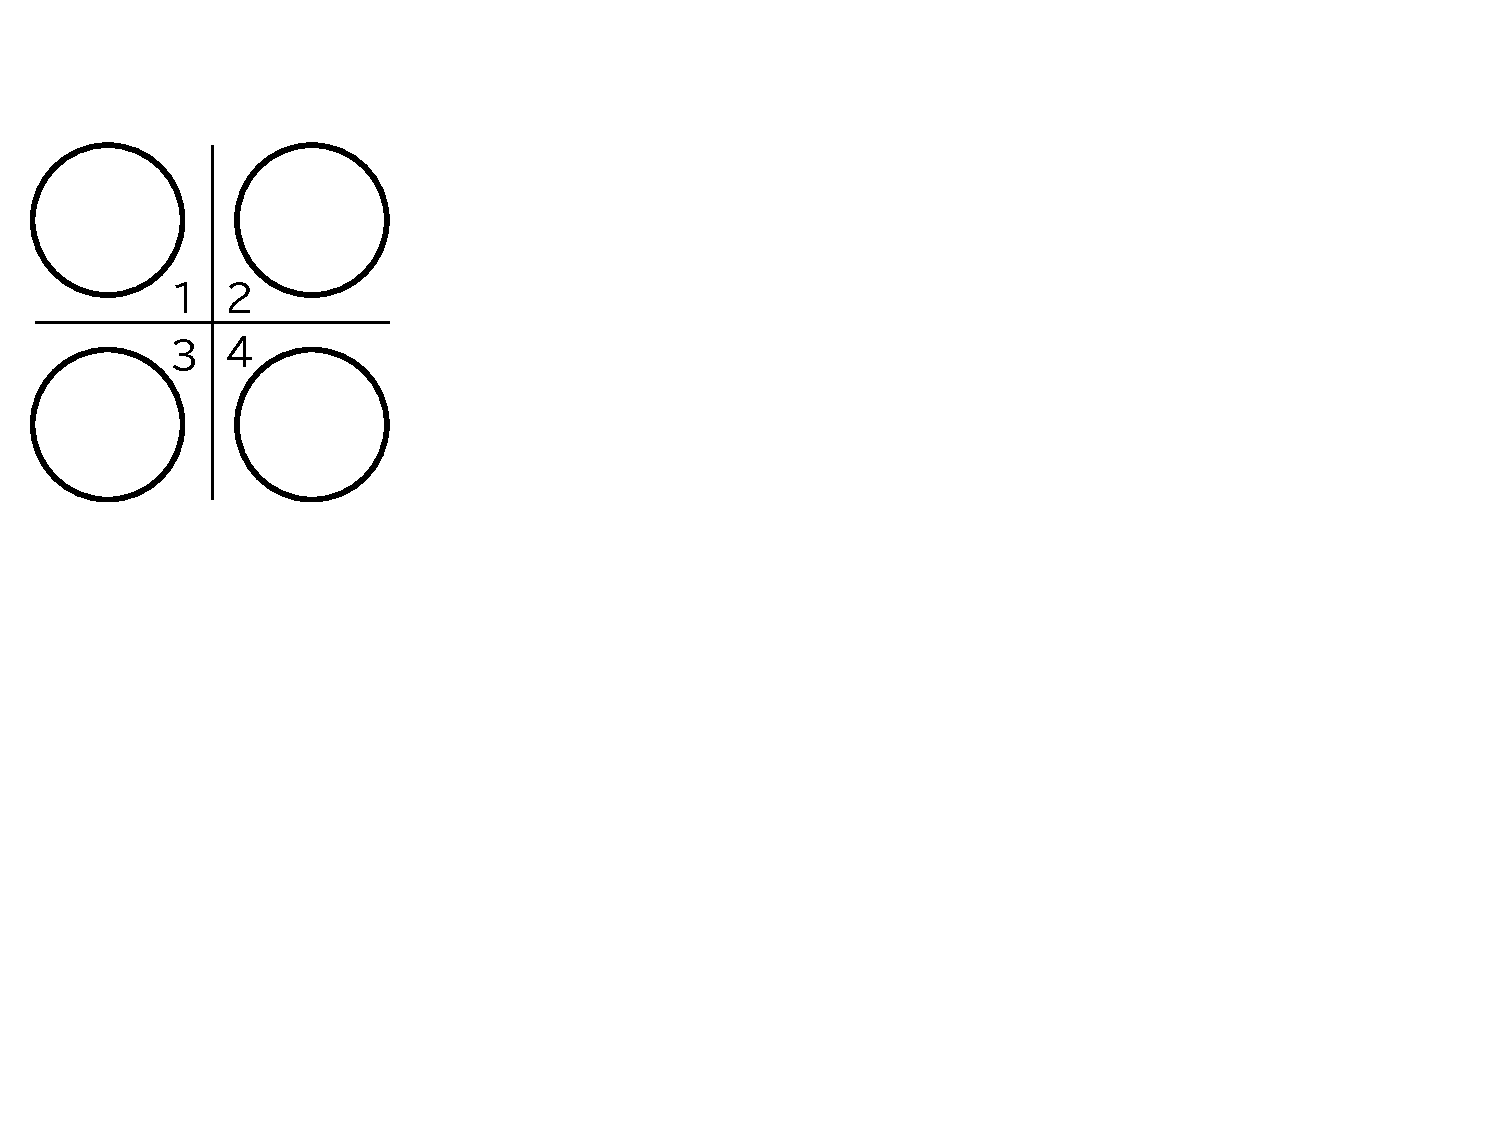
\includegraphics[width=3cm]{f1.pdf}
\end{wrapfigure}%
\mbox{}\\
\indent
2×2のマスにオセロの石を\textbf{白を上に向けて}置く。
各マスに番地をつけることで(左上のマスが1、右上のマスが2、左下のマスが3、右下のマスが4)、4つのマス(またはそこに置かれた石)を区別している\footnote{%
確率を考えるので、石を区別のつくものとしている。
}。

ここで、4つの石の中から無作為に1つ選び、それを裏返す。
その状態から、再び無作為に1つ石を選んでそれを裏返す(1回目に選ばれた石がもう一度選ばれてもよい)。
この試行を繰り返し、白と黒の数の遷移を調べよう。

図\ref{f:2}はこの試行を5回繰り返し、2→3→3→4→1という番地が選ばれたときの色の変化を表している。
\begin{figure}[] 
\centering 
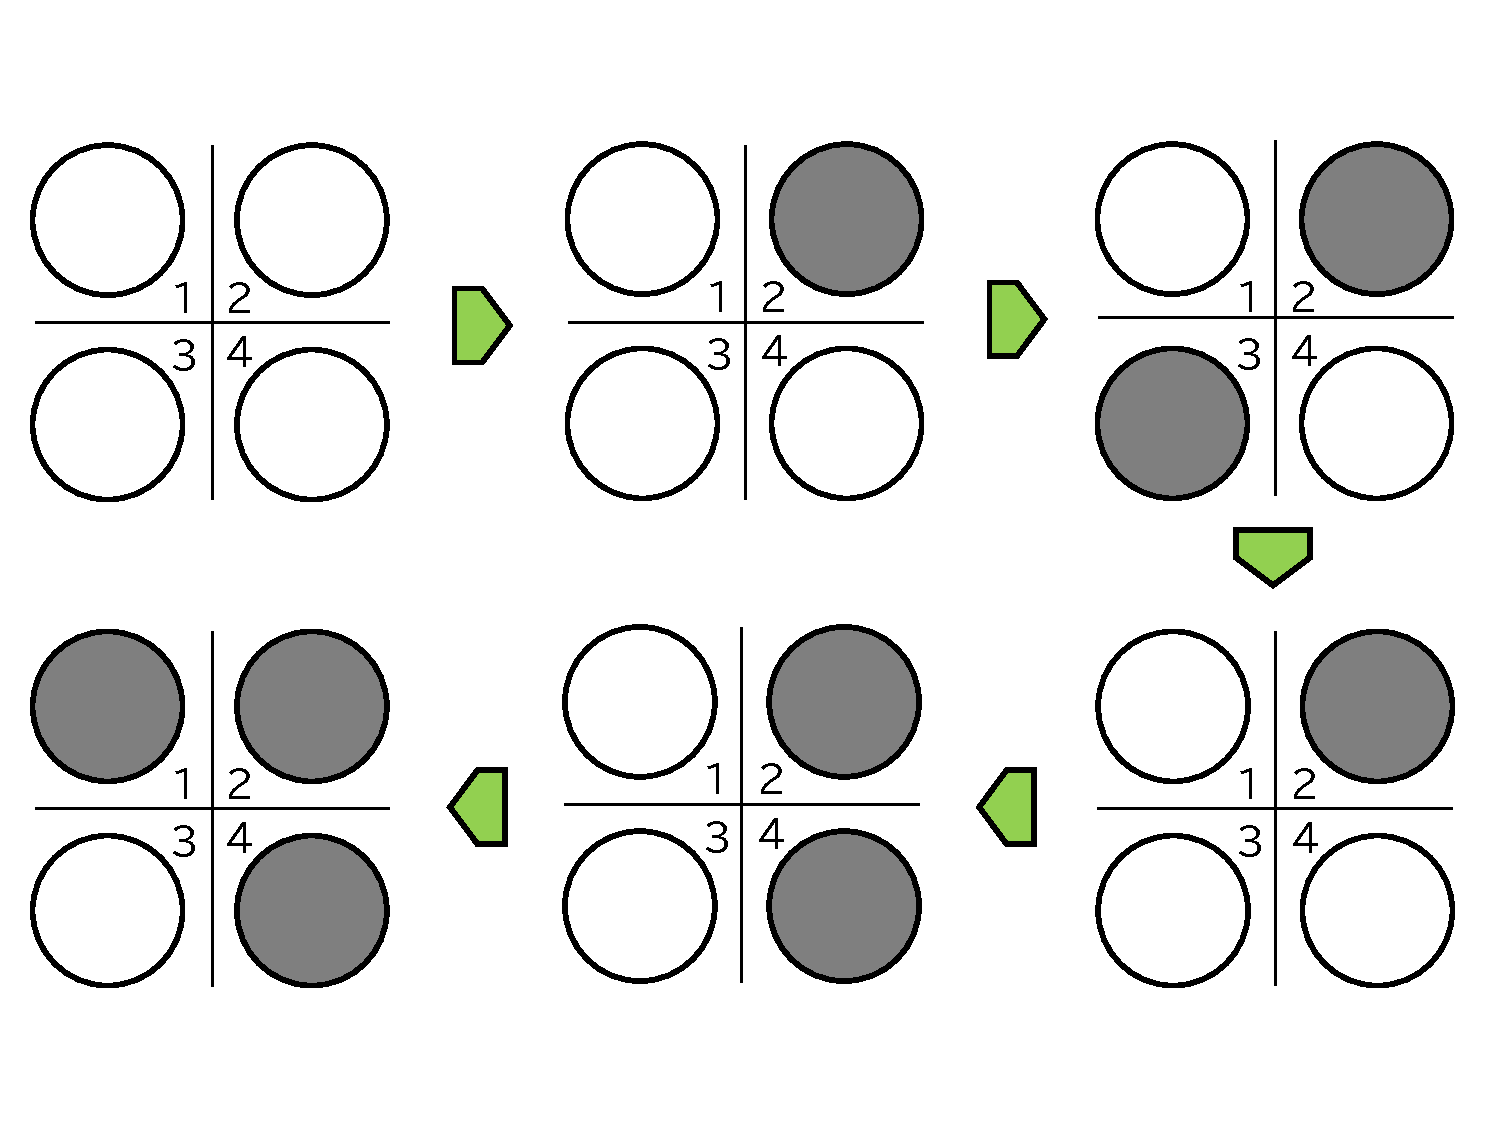
\includegraphics[width=10truecm]{f2.pdf}
\captionsetup{width=.9\linewidth}
\caption{%
2×2の石に5回の試行をおこなったときの色の変化の例。
はじめは4つとも白であった(上段左図)。
1回目の試行では番地2が選ばれたので、番地2の石は裏返され黒になった(上段中央図)。
2回目の試行では番地3が選ばれたので、番地3の石は裏返され黒になった(上段右図)。
3回目の試行では番地3が選ばれたので、番地3の石は裏返され白に戻った(下段右図)。
このように、1つ前の試行で操作されたばかりの石が再び裏返されてもよい。
4回目の試行では番地2が選ばれたので、番地4の石は裏返され黒になった(下段中央図)。
5回目の試行では番地2が選ばれたので、番地1の石は裏返され黒になった(下段左図)。
}
\label{f:2}
\end{figure}%

図\ref{f:2}の操作に関して、横軸を試行回数、縦軸を黒石の数として、石の移り変わりを表現したグラフを図\ref{f:3}に示した。
\begin{figure}[] 
\centering 
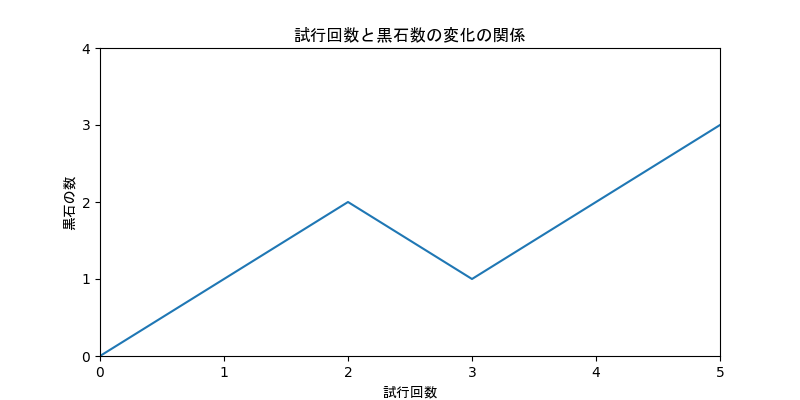
\includegraphics[width=14truecm]{f3.png}
\captionsetup{width=.9\linewidth}
\caption{%
図\ref{f:2}の操作における黒石数の変化を示したグラフ。
横軸を試行回数、縦軸を黒石の数とした。
}
\label{f:3}
\end{figure}%

\begin{enumerate}[(a)~]
\item \textbf{暇な人向けの問題}:
マス目が2×2だと特に面白くないから\footnote{%
こう言った理由はこの先の解説を聞けば分かるだろう。
}、4×4に設定を変更しよう。
実際に、オセロの石を16個用意し4×4に配置し、この試行をおこなってみよ。
もちろんオセロじゃなくても、表裏の区別がつくコインなどがあればそれで代用はできる。
最低でも50回は試行を繰り返してほしい\footnote{%
50回おこなうとだいたい石の色の遷移の特徴は見えてくる。
そういう理由で50回繰り返してほしいといった。}。
マスを無作為に選ぶ際には例えばグーグルの乱数ジェネレータ(\url{https://g.co/kgs/i7TXZL})などを用いればよい。
そして図\ref{f:3}を参考に、横軸に試行回数、縦軸に黒い石の個数を示すグラフをつくってみよ。
\end{enumerate}

今後の便を図って、記号を導入しておく。
舞台となるマスの個数(つまり、置かれる石の個数)を$N$とする。
例えば、2×2のマスであれば$N=4$である。
$N$個の石の中で、黒を上にして置かれている石の個数を$N^\mathrm{(b)}$と表す。
当然、$0 \le N^\mathrm{(b)} \le N$である。
上で説明した試行を計$n$回おこなうとする。

ここで、次のような2つの事象を考える:
\begin{align}
事象B:&~次の試行で黒石の数が増える。\notag \\
事象W:&~次の試行で白石の数が増える。\notag
\end{align}
今、全石の個数$N$の内、黒石が$N^\mathrm{(b)}$であるとき、次の試行で黒石の数が増える確率を$P_{N, N^\mathrm{(b)} } (B)$、次の試行で白石の数が増える確率を$P_{N, N^\mathrm{(b)} } (W)$と表す。

\begin{enumerate}[(a)~] \setcounter{enumi}{1}
\item \textbf{本節の要となる問題}:
(a)~と同じく、4×4のマス(つまり$N=16$)での操作を考える。
このとき、$N^\mathrm{(b)} = 0, 1, \dots ,N $の各値について$P_{N = 16,~N^\mathrm{(b)}} (B)$及び$P_{N = 16,~N^\mathrm{(b)}} (W)$を求めよ。
念のため日本語で表現すると、$P_{N = 16,~N^\mathrm{(b)}} (B)$は、計4×4=16個の石の内$N^\mathrm{(b)}$個が黒石であるとき、これまで説明してきた試行をおこなうと黒石が増える確率である。
(ヒント:
黒石数$N^\mathrm{(b)}$16通りあるが、確率の計算を$B,~W$それぞれについて16回ずつ繰り返す必要はない。
ここでの全事象は「次の試行によって黒石もしくは白石が増える」であるから、$\overline{B} = W$が言える。
よって、余事象の確率を利用できる。
)
\item \textbf{余力のある人向け}:
これまでと同じ4×4のマスで試行を$n$回おこなったときの黒石の個数$N^\mathrm{(b)}$の期待値$E [ N^\mathrm{(b)} ]$を求めよ。
\end{enumerate}

\paragraph{問題の解説}
\mbox{}\\
\indent
(a)~
50回の試行を繰り返し、すべての石が黒になる、またはすべて白になる(コインであればすべてが表もしくはすべてが裏になる)ことが滅多におこらないことを体感してほしかった。
さらに、石の数を増やして実験したら、石が一色にそろう頻度は増えるだろうか、減るだろうか。
予想してほしい。

(b)~
$N^\mathrm{(b)} = 0$のとき、16マスすべての石が白であるからどれを選んでも黒石の数は増える。
したがって、$P_{N = 16,~N^\mathrm{(b)} = 0} (B) = 1$である。
ヒントにも書いた通り、$\overline{B} = W$であるから、余事象の確率$P_{N = 16,~N^\mathrm{(b)} = 0} (W) = 1 - P_{N = 16,~N^\mathrm{(b)} = 0} (B)$を利用できる。
ゆえに、$P_{N = 16,~N^\mathrm{(b)} = 0} (W) = 1 - P_{N = 16,~N^\mathrm{(b)} = 0} (B) = 0$が求まる。
$N^\mathrm{(b)} = 1$のとき、16マスのうち15マスが白であり、この中から選べば黒石の数は増える。
したがって、$P_{N = 16,~N^\mathrm{(b)} = 1} (B) = \dfrac{15}{16}$である。
また、$P_{N = 16,~N^\mathrm{(b)} = 1} (W) = 1 - P_{N = 16,~N^\mathrm{(b)} = 1} (B) = \dfrac{1}{15}$が求まる。
$N^\mathrm{(b)} = 2$のとき、16マスのうち14マスが白であり、この中から選べば黒石の数は増える。
したがって、$P_{N = 16,~N^\mathrm{(b)} = 2} (B) = \dfrac{7}{8} ,~ P_{N = 16,~N^\mathrm{(b)} = 2} (B) = \dfrac{1}{8}$である。
結局コピペが続くだけなので、答えを表\ref{t:1}に並べて示した。
\begin{table}[]
\caption{$N = 4 \times 4$のマスに置かれた石の内、黒石の数$N^\mathrm{(b)}$が0, 1,..., 16それぞれ場合について、次の試行によって黒石の数が増える確率$P_{N = 16,~N^\mathrm{(b)}} (B)$と白石の数が増える確率$P_{N = 16,~N^\mathrm{(b)}} (W)$。}
\label{t:1}
\centering
\begin{tabular}{cccccccccccccccccc} \hline
$N^\mathrm{(b)}$ & 0 & 1 & 2 & 3 & 4 & 5 & 6 & 7 & 8 & 9 & 10 & 11 & 12 & 13 & 14 & 15 & 16 \\ \hline 
$P_{N = 16,~N^\mathrm{(b)}} (B)$ & 1 & $\frac{15}{16}$ & $\frac{14}{16}$ & $\frac{13}{16}$ & $\frac{12}{16}$ & $\frac{11}{16}$ & $\frac{10}{16}$ & $\frac{9}{16}$ & $\frac{8}{16}$ & $\frac{7}{16}$ & $\frac{6}{16}$ & $\frac{5}{16}$ & $\frac{4}{16}$ & $\frac{3}{16}$ & $\frac{2}{16}$ & $\frac{1}{16}$ & 0 \\
$P_{N = 16,~N^\mathrm{(b)}} (W)$ & 0 & $\frac{1}{16}$ & $\frac{2}{16}$ & $\frac{3}{16}$ & $\frac{4}{16}$ & $\frac{5}{16}$ & $\frac{6}{16}$ & $\frac{7}{16}$ & $\frac{8}{16}$ & $\frac{9}{16}$ & $\frac{10}{16}$ & $\frac{11}{16}$ & $\frac{12}{16}$ & $\frac{13}{16}$ & $\frac{14}{16}$ & $\frac{15}{16}$ & 1 \\ \hline 
\end{tabular}    
\end{table}

\paragraph{求めた確率について振り返る}\mbox{}\\
\indent

\begin{thebibliography}{99}
\bibitem{原} 原啓介:『測度・確率・ルベーグ積分 応用への最短コース』(講談社、2017年)。
\bibitem{ブラウン} 江沢洋、中村徹:『ブラウン運動』(朝倉書店、2020年)。
\bibitem{情報} 文部科学省ホームページの高等学校情報科「情報Ⅰ」教員研修用教材(本編)\url{https://www.mext.go.jp/a_menu/shotou/zyouhou/detail/1416756.htm}
\end{thebibliography}

\end{document}

%\begin{wrapfigure}{r}{3cm}\vspace*{-\intextsep}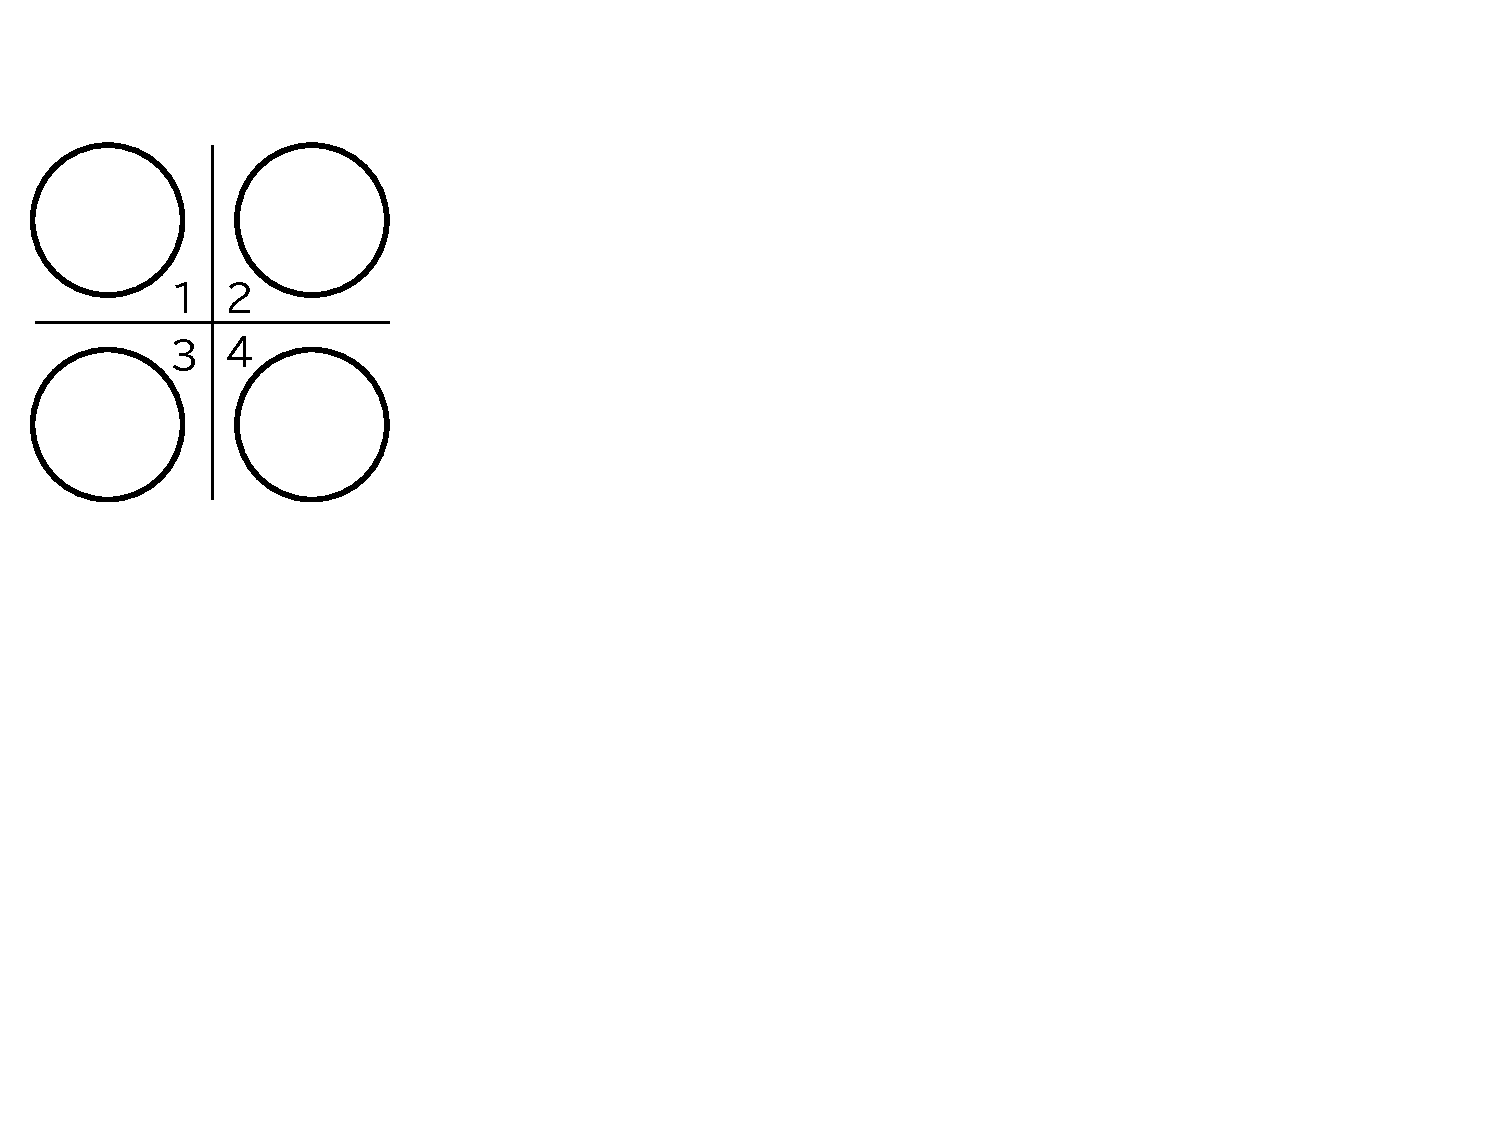
\includegraphics[width=3cm]{f1.pdf}\end{wrapfigure}